\documentclass{report}
\newcommand{\projectName}{SAP}
\usepackage[bookmarks=true]{hyperref}
\usepackage[dvipsnames, table]{xcolor}
\usepackage{graphicx} % Required for inserting images
\usepackage{tcolorbox}
\usepackage{multicol}
\usepackage{xcolor}
\usepackage{subfigure}
\usepackage{wrapfig}
\usepackage{longtable}
\usepackage[pages=some]{background}

\definecolor{lightgreen}{RGB}{237, 239, 234}
\definecolor{lightblue}{RGB}{234, 237, 239}
\definecolor{lightred}{RGB}{239, 234, 237}
\setlength{\arrayrulewidth}{1mm}
\setlength{\tabcolsep}{18pt}
\renewcommand{\arraystretch}{1.0}
\newcolumntype{s}{>{\columncolor[HTML]{AAACED}} p{9cm}}
\arrayrulecolor{Mahogany}

\RequirePackage{graphicx, pdfpages, pdflscape, pgfplots, tcolorbox, graphbox}

%
\usepackage[utf8]{inputenc}
\usepackage{titlesec}
\usepackage{eso-pic}
\usepackage[framemethod=tikz]{mdframed}
\usepackage[square,numbers]{natbib}
\AtBeginDocument{
  \renewcommand{\bibsection}{\chapter{\bibname}}
} % Bibliography in numbered chapter

\usepackage{geometry}
\usepackage{amsmath}
\usepackage{parskip}
\usepackage[official]{eurosym}
\setlength {\marginparwidth}{2cm} 
\usepackage{todonotes}
\usepackage{csquotes}

\usepackage{rotating}
\usepackage{lmodern}
\usepackage{setspace}


\hypersetup{
    %bookmarks=false,    % show bookmarks bar?
    pdftitle={Software Design Specification},    % title
    pdfauthor={Bharat-Krishn-Prathyush-Sujeeth},                     % author
    pdfsubject={\projectName Software Design Specification},                        % subject of the document
    pdfkeywords={SRS, client, use cases}, % list of keywords
    colorlinks=true,       % false: boxed links; true: colored links
    linkcolor=Dandelion,       % color of internal links
    citecolor=Bittersweet,      % color of links to bibliography
    filecolor=Periwinkle,        % color of file links
    urlcolor=PineGreen, % WildStrawberry        % color of external links
    linktoc=page            % only page is linked
}



\title{SWEProjectTeam18CoAP}
\author{Krishn Kher}
\date{\today}

\begin{document}
\setlength{\footskip}{50pt}
\BgThispage
% used packages in the template
% import your package here 


\begin{center}
\vspace*{1cm}

\backgroundsetup{
scale=1,
color=black,
opacity=0.15,
angle=0,
contents={%
  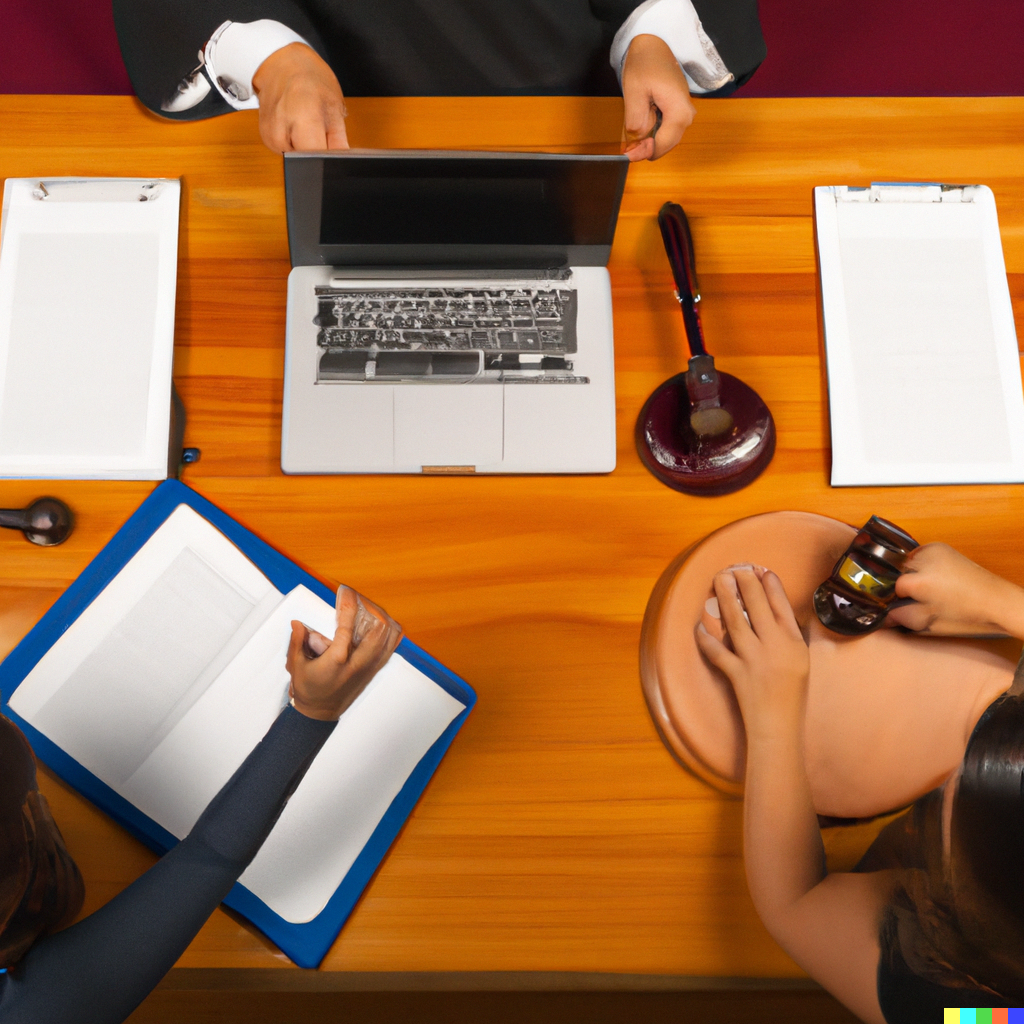
\includegraphics[width=\paperwidth,height=\paperheight]{images/SRS_Frontpage.png}
  }%
}

\begin{figure}[t]
  \raggedleft 
  \begin{minipage}{1cm}
  
\includegraphics[width=3cm]{images/IITH_Logo.png}
  \end{minipage}
\end{figure}

\vspace*{2cm}

\vspace*{0.1in}
%yellow version
\AddToShipoutPictureBG*{\AtPageLowerLeft{% 
  \color{OliveGreen}\rule{.16 \paperwidth}{\paperheight} }
   \:
   \:
   \;
   \;
   \:
  \begin{turn}{90} 
   \fontsize{35}{80}\selectfont \textbf{\color{SpringGreen} 
 ~\texttt{\projectName~SRS Documentation}}
  \end{turn}
  
  }

\begin{spacing}{1.7}

\begin{tabular}{p{4cm} ll}

& \textbf{\huge \projectName: Seat Allotment Portal}\\ % Here the title of your work \\
& \Large Software Requirements Specification \\ % Here the title of your work
& \\
& \large \textbf{\texttt{Course}}: Software Engineering \\
& \large \textbf{\texttt{Course code}}: \texttt{CS4443} \\

& \\
& \large \textbf{\texttt{Faculty Guide}}: \textit{Dr. MV Panduranga Rao} \\
& \large \textbf{\texttt{Student Developers}}: \\
& \large Bhavanam Sujeeth Kumar Reddy (\texttt{ES19BTECH11022}) \\
& \large Krishn Vishwas Kher (\texttt{CS19B23P000001}) \\
& \large Mukkavalli Bharat Chandra (\texttt{ES19BTECH11015}) \\
& \large Sree Prathyush Chinta (\texttt{CS19BTECH11043}) \\
& \\
& \\
& \begin{tcolorbox}[colframe=white, colback=Apricot, arc=8pt, boxrule=4mm, boxsep=1mm] \textbf{\texttt{Seat Allotment Portal}} tailored for managing CoAP/GATE admisssions @ IITH.
\end{tcolorbox} \\ 
\end{tabular}
\end{spacing}
\end{center}



\thispagestyle{empty} % Prevents page number from being included on the cover
\clearpage\setcounter{page}{1} % Start including page numbers from here
\pagenumbering{arabic} % in roman numerals
\tableofcontents
\clearpage

\chapter{Introduction}
\section{Purpose}
\begin{tcolorbox}[colframe=white, colback=lightblue, arc=8pt] Our system is designed to make it more convenient for the members of the student shortlisting committee dealing with the applications for PG programmes offered at the institute by allocating the seats to the students automatically with 100 \% accuracy.
This document provides specifications regarding the software architecture/design practices used in developing the said tool. The modules used in the architecture are delineated in chapter $1$.
The explicit architecture is depicted in chapter $2$. The intent is to create designs that accommodate useful modifications for various extra features. In the process of thinking extensively, we have made use of a couple of standard design patterns which we explain in chapter $3$. We also look into what sort of modifications our design patterns accommodate. Finally in chapter $4$, we summarize what possible modifications our design does not handle yet.\end{tcolorbox}

\section{Modules}

In this section we provide a list of all the modules accompanied by brief descriptions of each of them, as used in our software design. The modules have mostly been listed in the chronology of modules that would come into play as the user opens the tool and starts using it. \\\\
\newpage
\begin{longtable}{ |p{3cm}|s| }
\hline
\rowcolor{Melon} \multicolumn{2}{|c|}{\textbf{Core Modules}} \\
\hline
\rowcolor{lightgray}\textbf{Module Name} & \textbf{Synopsis} \\
\hline
\hline
\endfirsthead
\hline
\rowcolor{Melon} \multicolumn{2}{|c|}{\textbf{Core Modules (Cont'd)}} \\
\hline
\rowcolor{lightgray}\textbf{Module Name} & \textbf{Synopsis} \\
\hline
\hline
\endhead

\textit{Login} & This module defines which user has logged in and whether the user has logged out or not.\\
\hline
\textit{User} & This module defines the user that has logged in to the application. It stores data regarding the user, such as the set of projects created and which current project is opened.\\
\hline
\textit{Project} & This module describes what a project within the application looks like. It contains information regarding which round is currently being handled, the seat matrix, a set of auxiliary rules that the sort function uses to adjust the student data, and references to the set of UI observers so that appropriate changes in the project can be reflected in the UI.\\
\hline
\textit{Seat Matrix} & This module defines what seats are available and taken, for which specialization, and under which category.\\
\hline
\textit{Rule} & This module stores a set of auxiliary rules and their priority values so that the sort function in the project module can adjust the student data based on these auxiliary rules. \\
\hline
\textit{Auxiliary Rule} & This module defines which column and in what sort order should the student data be sorted.\\
\hline
\textit{UI Interface} & This is just the UI canvas where the application is viewed by the actor.\\
\hline
\textit{UI Decorator} & This module adds attributes to the UI handler based on the UI requirements. This module is the interface which every attribute that is added to the UI follows.\\
\hline
\textit{Dialog Box Decorator} & This module defines the dialog box UI attribute.\\
\hline
\textit{Drop Down Decorator} & This module defines the drop-down UI attribute. Several other modules like this can be defined to add to the UI interface.\\
\hline
\textit{Error Handler} & This module is defined to handle errors that occur in the application and notifies the user via the UI interface.\\
\hline
\caption{Modules in a synopsis.\label{ModulesList}}
\end{longtable}


\chapter{Diagrams}
\section{Structural View}
\subsection{Class Diagrams}
\begin{figure}[htp]
\href{https://www.canva.com/design/DAFfQlBz9aY/mV0XSkFn8OPFTq5QxdK9iw/view?utm_content=DAFfQlBz9aY&utm_campaign=designshare&utm_medium=link&utm_source=publishsharelink}{\fbox{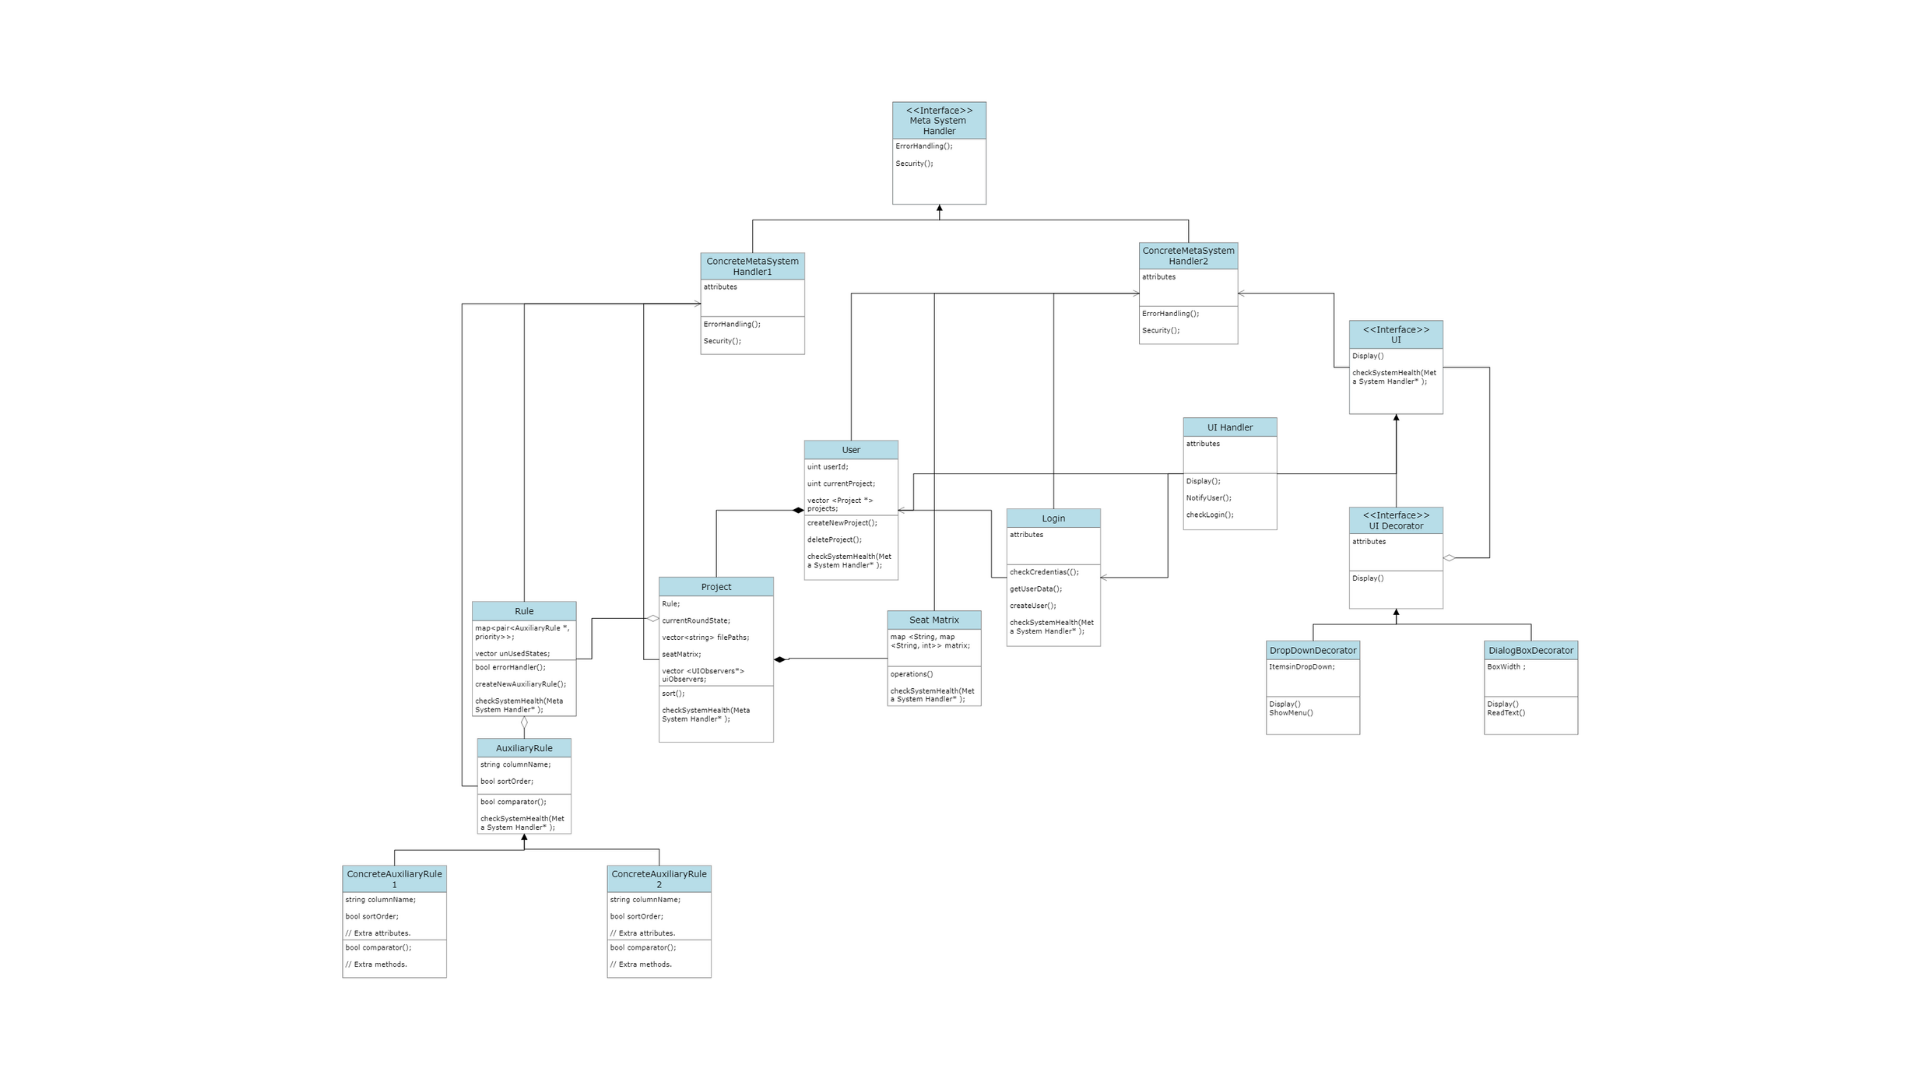
\includegraphics[width=15cm]{SD/images/Q2.png}}}
\caption{Class Diagram}
\end{figure}

\section{Behavioural View}
\subsection{Sequence Diagrams}
\begin{itemize}
    \item \textbf{Use Case $5$} \textit{Create Project
}\\
    \begin{itemize}
        \item \textbf{Primary Actor}: User.
        \item \textbf{Precondition}: User logged in.
        \item \textbf{Main scenario}: \begin{enumerate}
            \item User initiates the “Create Project” functionality. 
            \item System asks the user for the project name.
            \item User enters the project name.
            \item An empty project is created.
        \end{enumerate}
       \item \textbf{Alternate Scenario}: 
       \begin{enumerate}
           \item 
           \begin{itemize} 
           \item Project with the same name exists.
            \item System asks the user for a different name.
            \item User enters a different name.
            \item Empty project gets created.
           \end{itemize}
       \end{enumerate}
    \end{itemize}
\end{itemize} 
\begin{figure}[htp]
\fbox{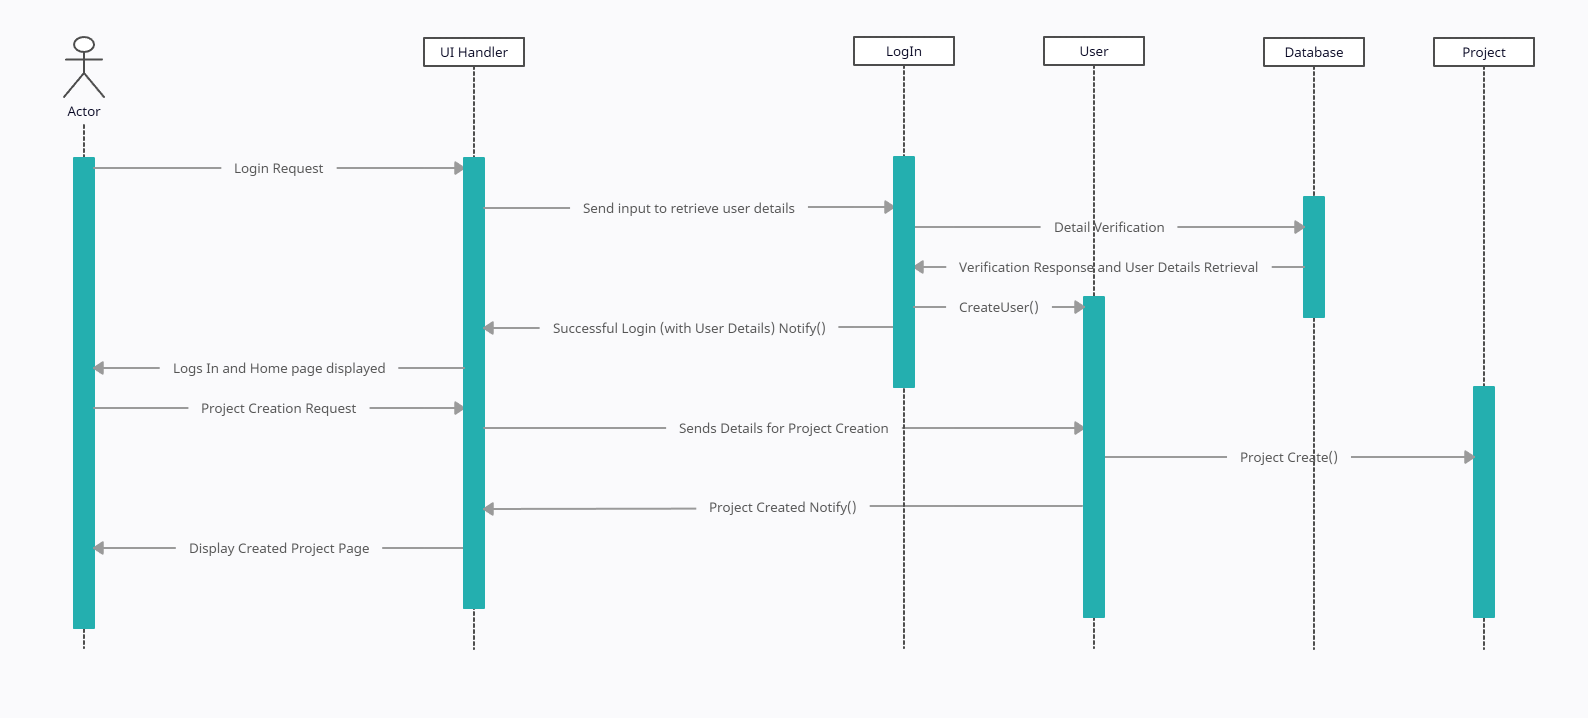
\includegraphics[width=15cm]{SD/images/SeqDiag1.png}}
\caption{Use Case 5 : Create Project}
\end{figure}
\newpage
\begin{itemize}
    \item \textbf{Use Case $10$} \textit{Uploading the Candidate Data in Round 1
}\\
    \begin{itemize}
        \item \textbf{Primary Actor}: User.
        \item \textbf{Precondition}: User has uploaded the seat matrix
        \item \textbf{Main scenario}: \begin{enumerate}
            \item User uploads the candidate data (csv file) on SAP. 
            \item The upload is successful.
            \item Preview of the uploaded csv file is shown on the screen.
        \end{enumerate}
       \item \textbf{Alternate Scenario}: 
       \begin{enumerate}
           \item 
           None
       \end{enumerate}
    \end{itemize}
\end{itemize}  
\begin{figure}[htp]
\fbox{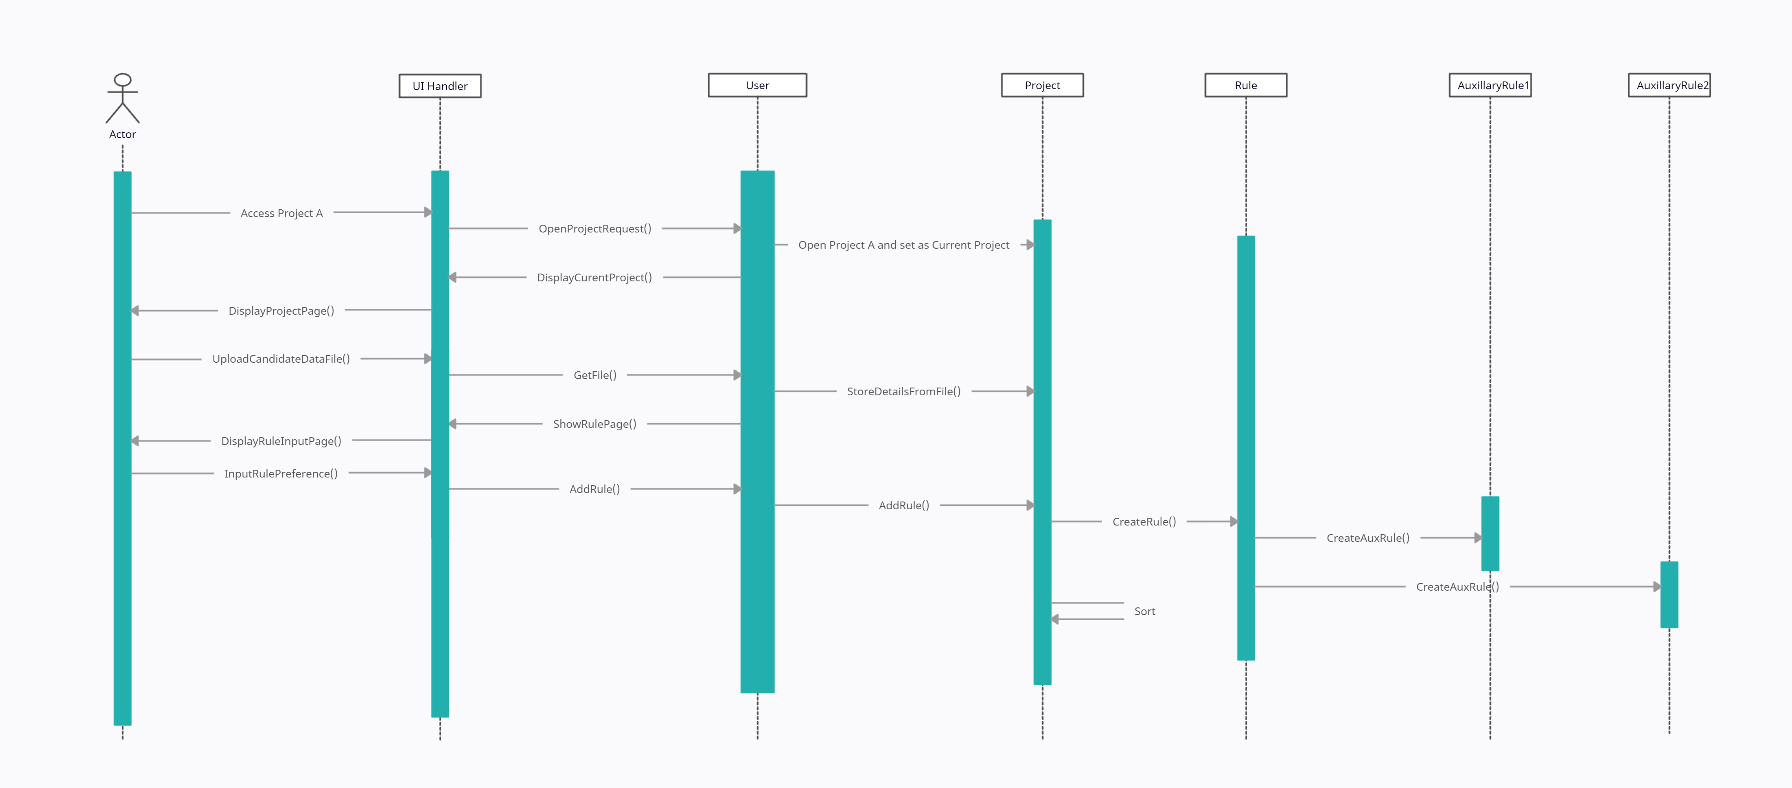
\includegraphics[width=15cm]{SD/images/SeqDiag2.png}}
\caption{Use Case 10 : Uploading the Candidate Data in Round 1}
\end{figure}

\newpage
\subsection{Activity Diagrams}
Deferred for further documentation in the future. Coming soon!
\section{Implementation View}
Deferred to later iterations of the development. Coming soon!
\chapter{Design Patterns}
\section{Philosophy}
Our applications of design patterns hasn't been one of pushing certain existing patterns blindly into the project! We created various sub-diagrams from different views in chapter $2$ to study different ways in which we can make the implementation and performance at run-time efficient. It so happened that the following design patterns were unearthed in the design process, as discussed below. Note that they span \texttt{Creational}, \texttt{Structural}, and \texttt{Behavioural} design patterns, which demonstrates the flexibility and organisation of our design.
\section{Applications}
As our sequence diagram in chapter $2$ suggest, our applications begin right with the \texttt{UI Interface} with which the user interacts! The UI being very user-friendly, hosts a range of facilities that a user may want to make use of, such as widgets, themes, scroll-bars (smooth scrolling), buttons, various text layouts, etc. In this context we employ the \textit{\textbf{Decorator}} pattern (cf. \ref{Appendix A}), using which we can dynamically add and remove layers of UI features to the raw page layout, efficiently. This approach has much support in precedent software projects. 
It also gives the developers the ability to flexibly add various features into the code without disturbing the services that other existing features offer in the UI. 

Our next usage of a design pattern again deals with the UI. Ideally we would like the user interface to notify the back-end modules depending on the buttons and options that the user selects. It then impels us to employ the \textit{\textbf{Observer}} pattern (cf. \ref{Appendix C}). Here, the subject is \texttt{UI Handler} and the observers are \texttt{User} and \texttt{Login}. The pages for \texttt{Login} are not necessarily dependent on the user, so we require the subject to notify the \texttt{Login} module separately. The need for the subject, \texttt{UI Handler} to notify \texttt{User} is self-explanatory. However it is to be noted that \texttt{UI Handler} does not require to inform \texttt{Project} and \texttt{Seat Matrix} separately since both have a composition relationship with \texttt{User} and \texttt{Project} respectively (similarly for the \texttt{Rules} class).
We also note that the \texttt{UI Interface} in the class diagram of chapter $2$ is not intended as an interface for the subject in the context of \textit{\textbf{Observer}} pattern but as an interface in the context of the \textit{\textbf{Decorator}} pattern. This is because we have only $1$ subject, so we do not require an interface just for $1$ concrete subject!

Guided by our sequence diagram, we now examine the phase of logging in to the portal. As we have seen in chapter $2$, this involves creating a \texttt{Login} object, which helps a user log in and logout into the system. Clearly, for each user's session, exactly one instance of a \texttt{Login} object is required. This rings a bell with a realization of the \textit{\textbf{Singleton}} pattern as described in \ref{Appendix D}, and we thus directly employ it here.

With respect to our creation of customized rules, we note an interesting hierarchy. A particular sorting rule is decomposed into auxiliary rules. In the particular context of our current use case, i.e., for CoAP, a rule consists of sorting across different columns in the XL sheet, including tiebreakers. An auxiliary rule would be a simple ascending/descending order-based rule on exactly $1$ column. This reminisces us of the \textit{\textbf{Factory Method}} pattern (cf. \ref{Appendix B}), where one has a factory that creates appropriate auxiliary rules and hands them over to the Rule class. While our current class diagram does not exactly follow this pattern, it resembles a usage of the same, thus making the creation of auxiliary rules more extensible, accurate, and manageable. Such auxiliary rules can be easily conglomerated in the \texttt{Rules} class.

Lastly, we examine the \texttt{Meta System Handler}, which is involved with practically all modules in our system. Its job is to perform error handling and security checks. We employ the \textit{\textbf{Visitor}} pattern (cf. \ref{Appendix E}) for this. The \texttt{Meta System Handler} provides the interface for various error-handling/security provisioning classes to perform checks for objects like \texttt{Project}, \texttt{User}, \texttt{Login},and \texttt{UI Handler}. 

Our analysis and study of design patterns yielded these design patterns as most relevant to our current software design, as compared to others.

\chapter{Future Extensions}
\begin{tcolorbox}[colframe=white, colback=lightblue, arc=8pt]
  The design so far has been made keeping various extensions in mind already. However, as mentioned in our \textit{SRS} document, various further improvements are possible, out of a few may not directly fit into the design pattern conceived of, as of now. The following are a few examples of the same:
  \begin{enumerate}
      \item Support for accessibility.
      \item NLP-based engine for generation of custom rules from plain human text.
      \item Concurrent transactions across multiple devices.
      \item Converting various input file formats into a common .csv file format and then passing the data to the core controller.
  \end{enumerate}
\end{tcolorbox}
\chapter{Appendix}
The below design patterns have been referenced from \href{https://www.amazon.com/gp/product/0201633612/ref=as_li_tl?ie=UTF8&camp=1789&creative=390957&creativeASIN=0201633612&linkCode=as2&tag=triatcraft-20&linkId=XRGUDJCGWC6AJNZM}{Design Patterns by Gang of Four}.
\section{Appendix A: Decorator Pattern}\label{Appendix A}
\subsection{Intent}
Attach additional responsibilities to an object dynamically. Decorators provide a flexible alternative to subclassing for extending functionality.
\subsection{Structure}
\begin{figure}[htp]
\begin{center}
    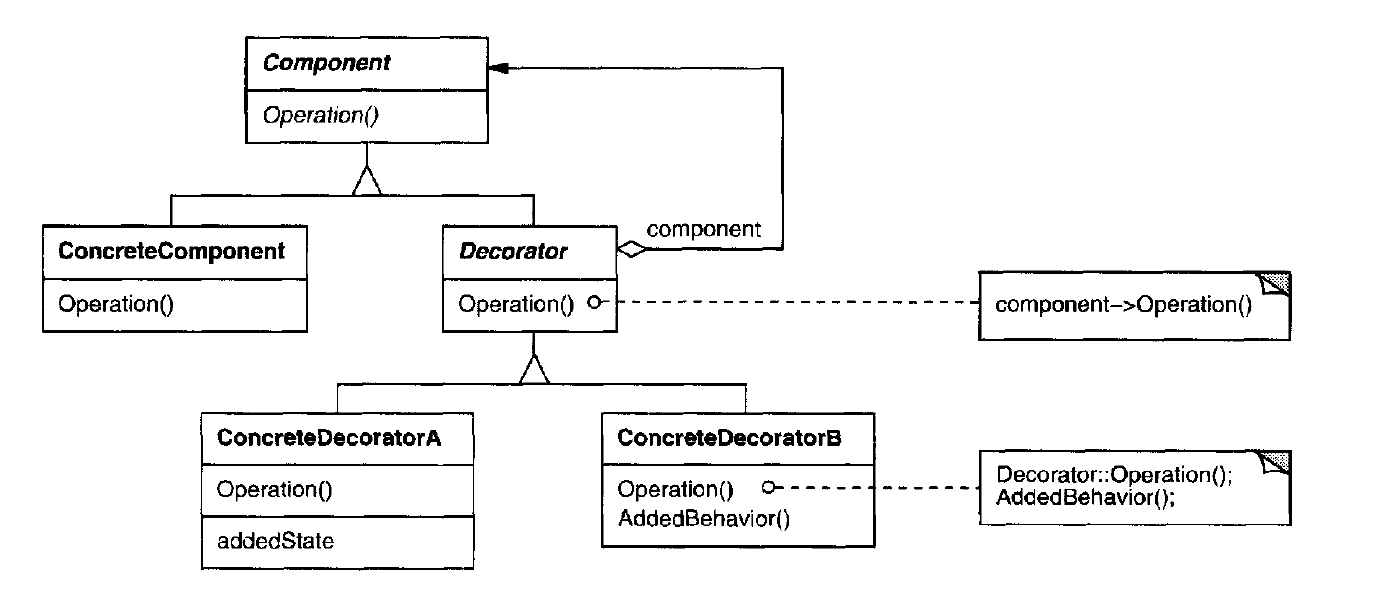
\includegraphics[width=10cm]{SD/images/deco-structure.png}
\end{center}
\end{figure}
\pagebreak
\section{Appendix B: Factory Method Pattern}\label{Appendix B}
\subsection{Intent}
Define an interface for creating an object, but let subclasses decide which class to instantiate. Factory Method lets a class defer instantiation to subclasses.
\subsection{Structure}
\begin{figure}[htp]
\begin{center}
    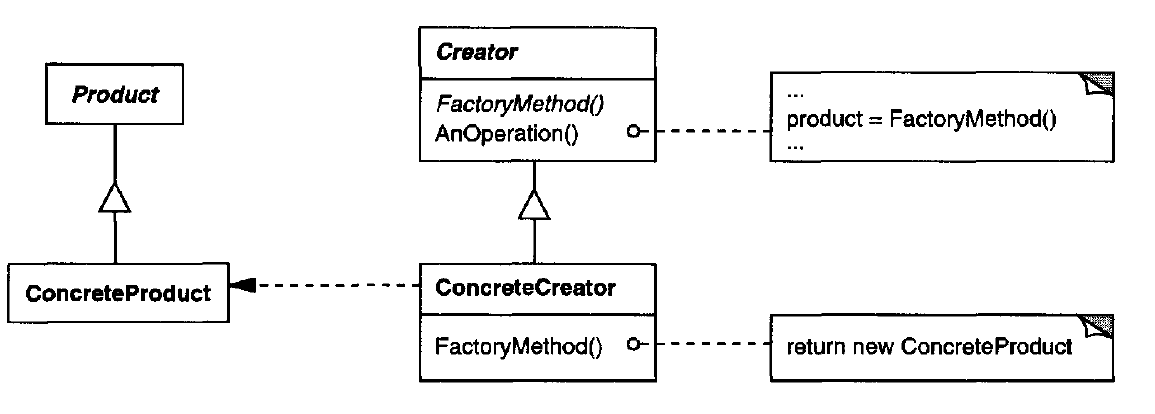
\includegraphics[width=10cm]{SD/images/fac-structure.png}
\end{center}
\end{figure}
\section{Appendix C: Observer Pattern}\label{Appendix C}
\subsection{Intent}
Define a one-to-many dependency between objects so that when one object changes state, all its dependents are notified and updated automatically.
\subsection{Structure}
\begin{figure}[htp]
\begin{center}
    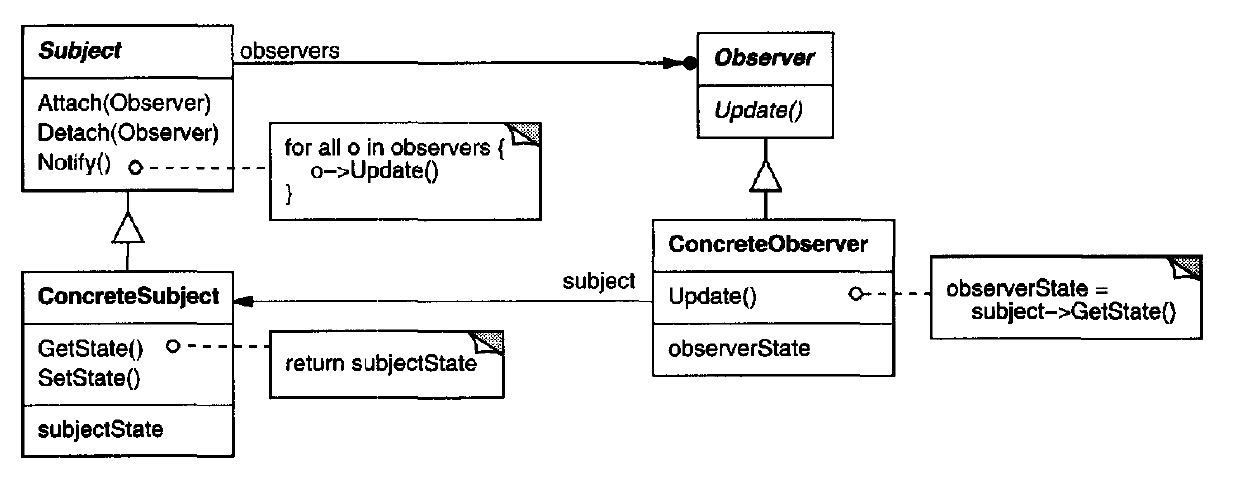
\includegraphics[width=10cm]{SD/images/obs-structure.png}
\end{center}
\end{figure}
\section{Appendix D: Singleton Pattern}\label{Appendix D}
\subsection{Intent}
Ensure a class only has one instance, and provide a global point of access to it.
\subsection{Structure}
\begin{figure}[htp]
\begin{center}
    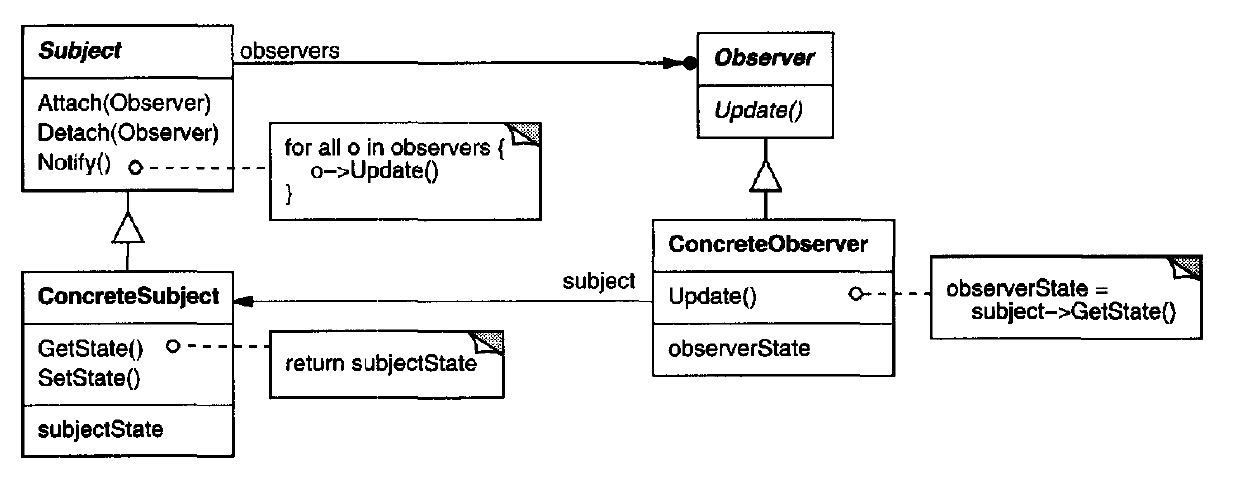
\includegraphics[width=10cm]{SD/images/obs-structure.png}
\end{center}
\end{figure}
\section{Appendix E: Visitor Pattern}\label{Appendix E}
\subsection{Intent}
Represent an operation to be performed on the elements of an object structure. Visitor lets you define a new operation without changing the classes of the elements on which it operates.
\subsection{Structure}
\begin{figure}[htp]
\begin{center}
    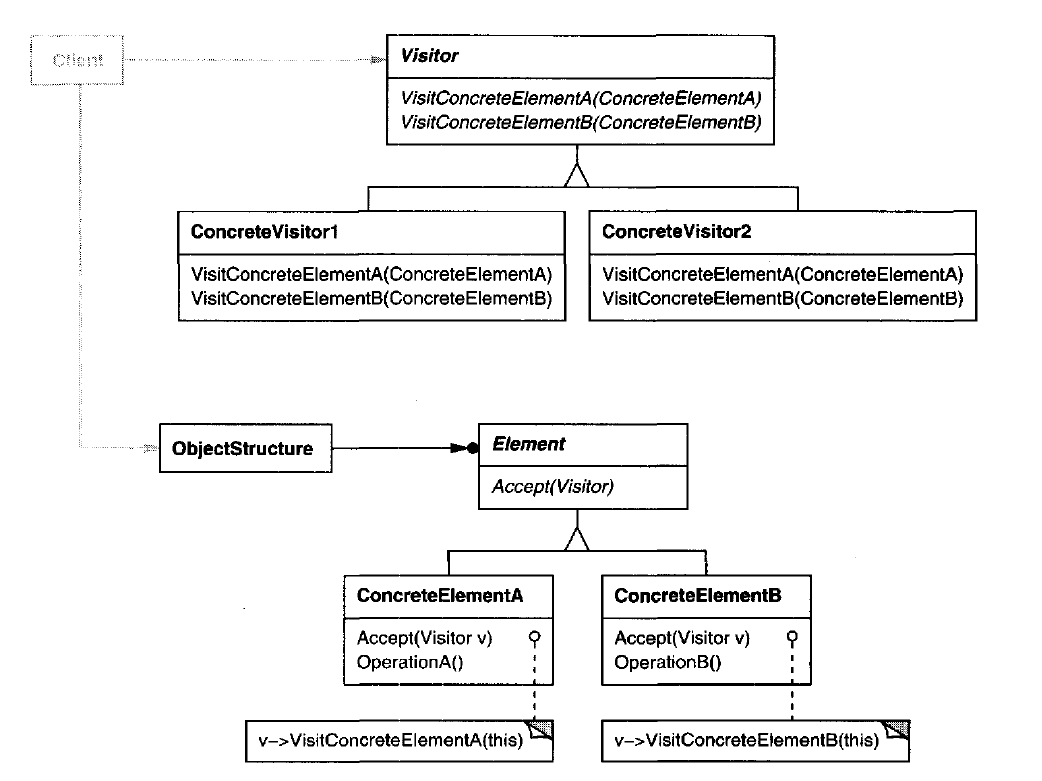
\includegraphics[width=10cm]{SD/images/vis-structure.png}
\end{center}
\end{figure}
\end{document}
